\documentclass[a4,12pt]{article}

\usepackage[utf8]{inputenc}
\usepackage[spanish]{babel}
\usepackage[margin=1.5cm]{geometry}
\usepackage{graphicx}
\usepackage{color}
\usepackage{import}
\usepackage{float }



\usepackage{hyperref}

\parindent 0em

%\usepackage{times}
\renewcommand{\familydefault}{\sfdefault}

\title{Breve introducción a GNU OCTAVE}
\author{Youssef Said Khloufi}
%\date{}

\begin{document}

\maketitle
\bigskip
\bigskip
\bigskip
\begin{figure}[H]
  \centering
    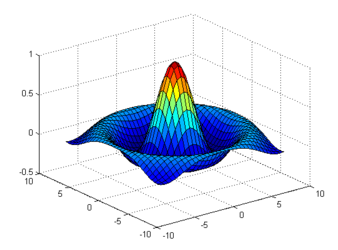
\includegraphics{graficos/octave}
\end{figure}
\newpage

\maketitle

\begin{abstract}
Este documento explica de manera muy breve los fundamentos y características principales del software libre GNU Octave.

\end{abstract}

\tableofcontents
\newpage

\section{Introducción}

OCTAVE : Lenguaje numérico de programación de libre acceso.

\subsection{Características principales del OCTAVE}

- Programa específico de Cálculo Numérico.\\
• Sólo opera con Números.\\
• Se puede considerar como una calculadora programable muy potente.\\
\medskip\\
-Programa muy popular entre estudiantes, ingenieros, técnicos e investigadores debido a sus características:\\
• Programa de libre acceso.\\
• Programa interactivo.\\
• Capacidades Gráficas sencillas.\\
• Posee gran cantidad de Funciones de todos los tipos.\\
• Lenguaje de programación de alto nivel similar a Fortran, C, Pascal o Basic, pero más  fácil de aprender.\\
Su lenguaje de programación es igual al de MATLAB.\\

\subsection{Acceso al OCTAVE desde el entorno Unix}

• Ejecutar la instrucción octave desde cualquier ventana\\
• Aparece la siguiente ventana del octave:\\
\begin{verbatim}
    octave:1>
\end{verbatim}

\subsection{Accesos al OCTAVE desde windows}

• Hacer doble click sobre el icono de OCTAVE.\\
• Al igual que en el entorno Unix , aparece la ventana del octave (consola).\\

\subsection{Algunas instrucciones de utilidad }

-pwd: nos dice en que directorio nos encontramos.\\
-ls: nos da una lista de los ficheros y los directorios\\
-cd: nombre nos permite cambiar al directorio nombre.\\

\subsection{Operaciones básicas.}

\begin{verbatim}
    + adición
    - sustracción
    * multiplicación
    ^ potenciación
    \ división izquierda
    / división derecha
\end{verbatim}

\begin{verbatim}
    exp   log   exponencial y logaritmo neperiano
    sin   cos   seno y coseno
    abs   sqrt  valor absoluto y raíz cuadrada
    round floor ceil funciones que redondean
\end{verbatim}

Ejemplos:

\begin{verbatim}
    > 2 + 3         > 2 * 2
    ans = 5          ans = 4

    > sin(pi/6)     > 2/6
    ans = 0.50000    ans =0.33333

    > log(5^3)      > round(4.5)
    ans = 4.8283     ans = 5

    > ceil(4.5)     > floor(4.5)
    ans = 5          ans = 4
\end{verbatim}

• Observe que: los () se reservan sólo para escribir el argumento de las funciones.\\

\subsection{Ayudas y normas generales del OCTAVE}

• El comando help nos proporciona información sobre las funciones del OCTAVE:\\
\begin{verbatim}
    > help round   % redondea al entero mas cercano
    > help floor   % redondea por defecto
    > help ceil    % redondea por exceso
\end{verbatim}
• Las flechas: arriba y abajo permiten recuperar comandos anteriores.\\
• Las flechas: izquierda y derecha permiten movernos a lo largo de una línea de instrucciones y corregirla.\\
• OCTAVE distingue entre mayúsculas y minúsculas:\\
\begin{verbatim}
    > ceil(2.3)
    ans = 3
\end{verbatim}
NO es lo mismo que:\\
\begin{verbatim}
    > Ceil(2.3)
    error: ‘Ceil’ undefined near line 22 column 1
\end{verbatim}
• Podemos asignar variables con determinados nombres a las expresiones numéricas (números,constantes).\\
\begin{verbatim}
    > m = 9.11e-31; q = -1.6e-19;
    > r = abs(q)/m
    r = 1.7563e+11
    > 3e+8
    ans = 300000000
    > m*(ans^2)
    ans = 8.1990e-014
\end{verbatim}
• Los nombres de estas variables pueden formarse utilizando letras,dígitos, etc.\\
• Las variables se pueden borrar con el comando clear nombre.\\
• Asignación por defecto: si a una expresión numérica no le asignamos un nombre, OCTAVE crea la variable ans.\\
• El comando who nos permite conocer los nombres de las variables asignadas. Ejecute who\\

\section{Vectores}

\begin{verbatim}
    vector: conjunto de números a1, a2, ..., an
\end{verbatim}

\subsection{Vectores fila y vectores columnas}

• Para definir vectores utilizamos los corchetes [ ].\\
• Los elementos de una fila se separan mediante espacios en blanco o comas .\\
• Los elementos de una columna se separan por puntos y comas o por nuevas líneas.\\
\begin{verbatim}
    > A=[ 1 2 3 4 5 6 7 8 9]; % vector fila
    > vecf=[1,2,3,4,5,6,7,8,9]; % vector fila
    > B=[ 1
    > 2
    > 3
    > 4 ]; % vector columna
    > vecc=[1;2;3;4]; % vector columna
\end{verbatim}
• El \% se utiliza en OCTAVE para escribir comentarios.

\subsection{Utilización de los dos puntos}

\subsection{Funciones sobre los vectores}

\subsection{Operaciones vectoriales y Operaciones puntuales}

\section{Editor del OCTAVE. Programación}

\subsection{Tipos de m-files}

\section{Secuencias}

Una forma sencilla de producir una secuencia de números es utilizando la notación n:m
donde n es el número inicial y m el final

\begin{verbatim}
	octave:2> 1:10 ans =

	1	2	3	4	5	6	7	8	9	10
\end{verbatim}

También podemos usar la notación p:q:r para crear una secuencia que inicia en p, finaliza en r con intervalos de q. En el siguiente caso almacenaremos en una variable b una secuencia partiendo de cero y finalizando en diez, con un intervalo de dos entre cada número.

\begin{verbatim}
	octave:3> b=0:2:10 b =

	0	2	4	6	8	10
\end{verbatim}

Tenemos	otras	dos	funciones	que	nos	permiten	crear	vectores	de	elementos secuenciales,  estos  son  linspace y  logspace,  el  primero  separa  los  números uniformemente y el segundo lo hace logarítmicamente.

\begin{verbatim}
	octave:39> linspace(1,4,6)
	ans =

	1.0000	1.6000	2.2000	2.8000	3.4000	4.0000
\end{verbatim}

\section{Gráficos}

\subsection{Gráficos en 2 dimensiones}

\subsection{Gráficos en 3 dimensiones}

Para producir gráficos en 3D disponemos de varias opciones, la mas simple es usar el comando  plot3(x,y,z) donde cada argumento es tomado para convertirse en los vértices del gráfico tridimensional.

Si todos los argumentos son vectores de la misma longitud se dibujará una única línea continua. En caso de todos los argumento sean matrices cada una de las columnas de las matrices serán tratada como líneas separadas.

En caso de que sólo se le pasen dos argumentos en lugar de tres, plot3(x,c), el segundo argumento 'c' debe ser un número complejo, así, las partes reales e imaginarias de éste son usadas como las coordenadas y e z respectivamente.

Si sólo se le pasa un argumento, plot3(c), las partes reales e imaginarias de los argumentos son usados como los valores y y z, y se trazan frente su índice.

El comando plot3 también acepta los argumentos que permiten modificar el formato de presentación de la gráfica descritos en la sección de gráficas bidimensionales.

Ejemplo:\\
\begin{verbatim}
	octave:51> z = [0:0.05:5];
    octave:52> plot3(z, exp(2i*pi*z), "3;sinusoidal compleja;")
\end{verbatim}
\begin{figure}[H]
  \centering
    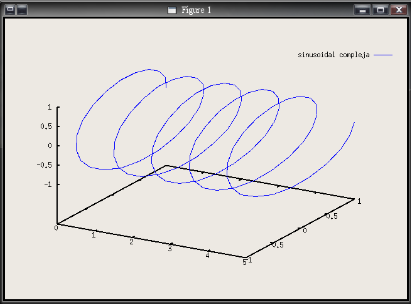
\includegraphics{graficos/imagen4}
  \caption{Gráfica de una sinusoidal compleja con 'plot3()'}
\end{figure}

El comando mesh(x,y,z) hace una representación tridimensional dado dos vectores x e y,  y  una  matriz  bidimensional  z.  Generalmente  se  usa  el  comando  meshgrid para generar los datos que usará mesh para para representar los ejes x e y.

Ejemplo:\\
\begin{verbatim}
	octave:1> x=[-2:0.1:2];	% genera el vector
	octave:3> [xx,yy] = meshgrid(x,x);	% genera las matrices de ejes octave:4> z=sin(xx.^2 – yy.^2);	% funcion z=sen(x^2 – y^2) octave:5> grid	% genera una rejilla
	octave:6> mesh(x,x,z)	% crea el grafico
\end{verbatim}
\begin{figure}[H]
  \centering
    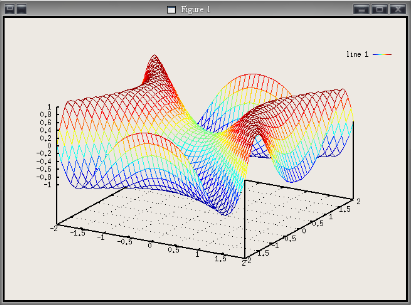
\includegraphics{graficos/imagen5}
  \caption{Generación de gráficos mediante 'mesh()'}
\end{figure}

La función contour(x,y,z) recibe los mismos argumentos que mesh() y dibuja las curvas de nivel de la superficie.

Vamos a generar las curvas de nivel del gráfico generado en el ejemplo anterior:

\begin{verbatim}
	octave:10> contour(x,x,z);
\end{verbatim}
\begin{figure}[H]
  \centering
    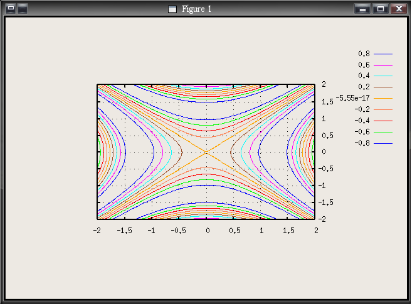
\includegraphics{graficos/imagen6}
  \caption{Curvas de nivel generadas por medio de 'contour()'}
\end{figure}

\section{Grabar y leer datos en ficheros. Impresión de las gráficas}

\end{document}
